% ****** rbf.tex ******
% Este archivo provee el formato para la Revista Boliviana de Fisica, RBF.
\documentclass{rbf}
%\documentclass[onecolumn]{rbf}

\usepackage{amsmath}
\usepackage[utf8]{inputenc}
%\usepackage[latin1]{inputenc}
\usepackage{url}
\usepackage{apacite}

\begin{document}

\title{ESTUDIO DEL MÉTODO MONTE CARLO EN SIMULACIONES PARA LA ESTIMACIÓN DEL VALOR DE PI}

\author{Juan Pablo Crespo Vargas\marca{*}}
\afil{Sensei Dojo Cobra Py, https://github.com/CobraPython}%

\alpie{*}{jp.crespo.vargas@gmail.com}% Las lineas se cortan automaticamente o puede obligarse esto con

\author{Carlos CCC \marca{**}}
\afil{Sensei 2 Dojo Cobra Py, https://github.com/CobraPython}%

\alpie{**}{ccc@gmail.com}% Las lineas se cortan automaticamente o puede obligarse esto con

\begin{abstract}
\Resumen
En este artículo se presenta los resultados de tres metodologías diferentes en las que se aplicó una simulación Monte Carlo para estimar el valor de Pi: el método de comparación de áreas, el método propuesto por Buffon y la extensión de Laplace. Los tres casos se desarrollaron en un lenguaje de alto nivel, Python y la librería Numpy que le otorgan un performance optimizado. Se estudió con detalle el resultado no determinista de las simulaciones y se demostró que cumplen con los teoremas fundamentales de la probabilidad.

\descriptores{Simulación, Monte Carlo, Pi, Buffon, Buffon-Laplace, Python, Numpy}


\Abstract
This article represents the result of three different metodologies for estimate the pi value with Monte Carlo's simulation: the comparition area's method, the method proposed by Bufffo and the Laplace's extention. The three cases had been developed in  Python ( high level language) and Numpy library which give it an optimized performance. The non-deterministic result of the simulations was studied in detail and it was shown that they comply with the fundamental theorems of probability.

\keywords{Biographies, tributes, personal notes -- Control of chaos, applications of chaos}
\end{abstract}

\maketitle

%%%%%%%%%%%%%%%%%%%%%%%%%%%
%   INTRODUCCION
%%%%%%%%%%%%%%%%%%%%%%%%%%%

\section{Introducción}\label{intro}
El método de Monte Carlo tiene un génesis moderno en el trabajo pionero de Stan Ulam y John Von Neumann. Luego de la segunda Guerra Mundial aplicaron distintos métodos de Monte Carlo en simulaciones para el desarrollo de armas termonucleares. Desde entonces y por más de 50 años que se aplicaron estos desarrollos en la investigación y perfeccionamiento de distintos métodos que modelan el transporte de neutrones y radiación gamma con bastante éxito experimental\cite{Kling}. 

Hoy resulta una alegre ironía que ningún producto que haya aplicado la metodología Monte Carlo en su desarrollo, se haya empleado en conflicto alguno. Más aún los científicos han explotado el uso de simulaciones Monte Carlo para obtener un beneficio público positivo aplicándola en salud. Por ejemplo, los planeamientos de dosis en radioterapia dependen actualmente en algún grado de cálculos obtenidos mediante simulaciones que emplean Monte Carlo.


El método de Monte Carlo es un método de resolución numérica donde se modelan las relaciones e interacciones de distintos objetos y su entorno, mediante la generación aleatoria de estas interacciones. Mientras mayor sea la repetición de pruebas se obtiene un resultado que va convergiendo a un valor con mayor precisión. Es por el recurso de la aleatoriedad que obtiene el nombre Monte Carlo, pues se inspira en la región del Principado de Mónaco donde se encuentran el casino Monte Carlo.
Un método Monte Carlo se puede definir de la siguiente forma: <<Los métodos Monte Carlo son aquéllos en los que las propiedades de las distribuciones de las variables aleatorias son investigadas mediante la simulación de números aleatorios. Estos métodos, dejando a un lado el origen de los datos, son similares a los métodos estadísticos habituales en los cuales las muestras aleatorias se utilizan para realizar inferencias acerca de las poblaciones origen. Generalmente, en su aplicación estadística se utiliza un modelo para simular un fenómeno que contiene algún componente aleatorio. En los métodos Monte Carlo, por otro lado, el objeto de la investigación es un modelo en sí mismo, y se utilizan sucesos aleatorios o pseudoaleatorios para estudiarlo.>>\cite{Gentle}


El método cobra una especial relevancia las
últimas décadas debido a que se produjeron
sustanciales y significativos avances respecto a la
potencia de los procesadores y las distintas
arquitecturas informáticas. Es ampliamente usado
en problemas donde obtener un resultado
analítico no es posible, o en problemas que
contienen demasiada complejidad (como es el
caso de la ecuación de transporte de Boltzmann
para partículas sin carga).\cite{Kling}


%%%%%%%%%%%%%%%%%%%%%%%%%%%
%   midelo de simulacion
%%%%%%%%%%%%%%%%%%%%%%%%%%%

\section{Modelo de Simulación.}
\subsection{Entorno de desarrollo}

Como quedo manifiesto en el anterior punto el método Monte Carlo tiene una precisión proporcional a $\frac{1}{\sqrt{N}}$. En comparación con otros métodos numéricos determinísticos (como por ejemplo el método de trapecios o Simpson para encontrar la integral de una función definida) que tienen un error de aproximación proporcional a $\frac{1}{N^2}$ en el mejor de los casos, los métodos que aplican Monte Carlo (como por ejemplo la integración por Monte Carlo) requieren una cantidad considerable mayor de datos a procesar. Sumado este hecho a la complejidad que puede involucrar el modelamiento de las interacciones aleatorias, es que generalmente se prefiere usar lenguajes de programación de bajo nivel que permitan optimizar el tiempo de cómputo total.

Por ejemplo, es común encontrar desarrollos en c, c++ y Fortran entre otros. Existiendo hoy librerías que facilitan la generación de números pseudoaleatorios y el manejo matemático. Aún con esta ventaja el código necesario para una aplicación final suele ser bastante complicado y extenso.
Estos dos criterios identificados se consideraron para la selección del entorno de desarrollo:

1. El tiempo de procesamiento.
2. La legibilidad y simplificación en el código.

Siendo Python un lenguaje de alto nivel que cumple con el segundo criterio, al incluir la librería Numpy (librería de procesamiento numérico para Python) obtenemos una velocidad de procesamiento comparable a C. Adicionalmente se utilizó una librería para la representación de los datos, Matplotlib.
Se detalla todo el código y las dependencias en el repositorio del proyecto:

https://github.com/CobraPython/montecarlopi

\subsection{Generación de números Pseudeoaleatorios}

Existen distintos métodos para la generación de números aleatorios, sin embargo, la generación de estos en ordenador parte necesariamente desde una semilla (seed) que es un valor concedido por el usuario. Con esta semilla se genera una única serie de números aleatorios, pudiendo ser replicados a partir de esta. Por esta razón es que se denominan números pseudo aleatorios.
La librería Numpy utiliza el algoritmo Mersenne Twistter (MT19937) \cite{Tanguy} para la generación de números pseudoaleatorios. Este método particular tiene la cualidad de tener una periodicidad bastante grande en la generación de números: $2^{19937}−1$\cite{Makoto}.

\subsection{Métodos de estimación de Pi}
\subsubsection{Método Simple para la estimación de Pi}

Se propone estimar el número de Pi con el siguiente modelo:
Consideramos un cuadrado de lado L, con una circunferencia en su interior de radio L.
La relación de áreas se da en la ecuacion \ref{areaseq}:

\begin{equation}
	\frac{A_{circunferencia}}{A_{cuadrado}}=\frac{\pi L^2}{L^2}
\label{areaseq}	
\end{equation}}

Una forma de calcular esta relación de áreas es lanzar al azar puntos dentro del cuadrado. Estos puntos pueden quedar también dentro de la circunferencia, la relación de áreas quedara expresada por aquellos puntos que estén dentro del circulo sobre el total.
En la gráfica \ref{area} se muestra un ejemplo del experimento propuesto, mostrando un solo cuadrante ya que las áreas son simétricas en cada eje.

\begin{figure}[htbp!]
 \centering
  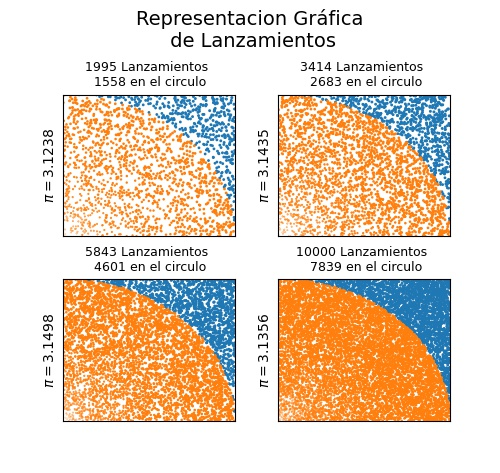
\includegraphics[width=0.4\textwidth]{figures/areas.jpg}
	\caption{Representación gráfica de la estimación de Pi mediante el lanzamiento aleatorio de puntos. Mientras mayor sea el número de lanzamientos las áreas son más definidas}
 \label{area}
\end{figure}

Queda bastante ejemplificado que mientras mayor sea el número de puntos, las áreas quedan mejor definidas.
Para obtener esta aproximación se necesitan generar los puntos aleatoriamente con una distribución uniforme, es decir, con igual probabilidad de caer dentro y fuera del área del cuarto de circunferencia.

\subsection{Método de Buffon para la estimación de Pi}

En el caso de la estimación de Pi usando la propuesta experimental de Buffon y su extensión de Laplace tenemos más variables aleatorias a considerar. Puesto que cada aguja cae aleatoriamente con un centro en $(𝑥_𝑖,𝑦_𝑖)$, tiene relacionada otra variable aleatoria que corresponde al ángulo de inclinación $\theta$ de la aguja. La figura \ref{aguja} nos muestra un ejemplo.



\begin{figure}[tbp!]
 \centering
  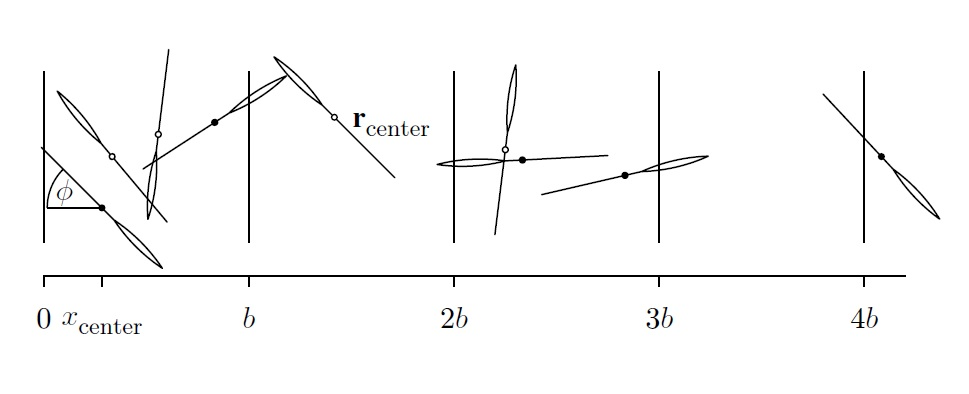
\includegraphics[width=0.4\textwidth]{figures/agujas.jpg}
	\caption{Las agujas caen en una posición y ángulo aleatorio. Dependiendo de este ángulo se puede determinar si la aguja cruza una línea.\cite{Statistics}}
 \label{aguja}
\end{figure}

Si bien en este caso se recurre a una función trigonométrica para evaluar la inclinación y considerar a las agujas que cruzan la línea, el ordenador usa recursivamente el valor de Pi para calcular la función coseno, siendo este un error “histórico” ya que recurre al valor de pi para calcular al mismo. Por esta razón se usó una corrección geométrica que evita el uso de funciones trigonométricas.

Pasando de requerir generar aleatoriamente un ángulo $\theta$, a generar aleatoriamente desplazamientos $\delta x$,$\delta y$. En la siguiente figura se muestra una representación gráfica de cómo se realiza la simulación con un número grande de lanzamientos aleatorios con distribución uniforme. \cite{Statistics}

Para esta propuesta del lanzamiento de agujas para la estimación de Pi, se comparan dos casos:
-Problema Buffon, cuando las agujas cruzan líneas en un solo eje.
-Problema Buffon-Laplace, cuando las agujas cruzan líneas en sentido vertical y horizontal.




\begin{figure}[tbp!]
 \centering
  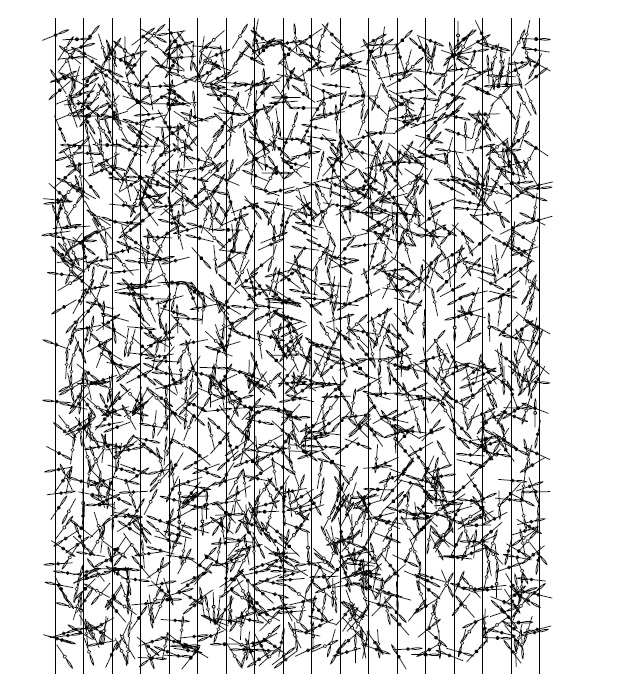
\includegraphics[width=0.4\textwidth]{figures/buffon.jpg}
	\caption{Representación gráfica del experimento de Buffon lanzando 2000 agujas.\cite{Statistics}}
 \label{buff}
\end{figure}


En la figura \ref{buff} se puede ver el resultado del lanzamiento de 2000 agujas de largo $a$ de la misma longitud que la separación de las lineas $b$, es decir que $a=b$. La probabilidad se calcula en relación a cuantas agujas cruzan una línea sobre el total de agujas. 



\section{Epílogo}\label{epi}
Como el lector habrá percibido durante la lectura de esta entrevista, la teoría del caos continúa siendo una de las pasiones de JY lo que le permite transmitir de manera didáctica los conceptos ligados a la misma. Es uno de los artífices de los conceptos desarrollados por el prestigioso grupo de caos de la universidad de Maryland descrito en \cite{UMD17}, y entre los que también se cuentan a Edward Ott, Celso Grebogi, Rajarshi Roy entre otros y también a colaboradores dentro de su propia institución como Eugenia Kalnay así como externos, entre los que mencionamos a Jason Gallas\footnote{Tanto Kalnay como Gallas están ligados a la RBF por ser o haber sido parte del Comité Editorial.}.

\begin{acknowledgments}
Agradezco al MPIPKS por haber posibilitado mi participación en el taller ``Multistability and Tipping: From Mathematics and Physics to Climate and Brain". A Sergio Yañez Pagans (hoy en la Universidad de Arizona) por el excelente trabajo de edición del vídeo de la entrevista y por su permanente entusiasmo en las actividades científicas. A Fernando Poma Ajoruro por haber realizado parte de la transcripción y por la permanente colaboración que brinda al Grupo de Sistemas Complejos de la UMSA.
\end{acknowledgments}





\bibliographystyle{apacite}
\bibliography{bibliografia.bib}{32}
\end{document} 